\documentclass{article}
\usepackage[utf8]{inputenc}
\usepackage{amsmath}
\usepackage{amssymb}
\usepackage{enumitem}
\usepackage[hidelinks]{hyperref}
\usepackage{multicol}
\usepackage{tabularx}

\usepackage{tikz}
\usetikzlibrary{decorations.pathmorphing}

\title{CS 40 Homework 5}
% Yeah, this is a hack...
\author{Due Monday, February 27th}
\date{Winter 2023}

\begin{document}

\maketitle

\noindent
A note on proofs:
Make sure you state what you're proving, what proof method you're using, and---once your proof is complete---what your conclusion is.
If you use induction, make sure to label your base case and your inductive case.
If you use a lot of symbols, a summary of your approach may be helpful to the reader.


\section{Cubes}

Prove that the following equation is true for all natural numbers.
Use induction.

$$\sum_{i=0}^n i^3 = \left(\frac{n^2 + n}{2}\right)^2$$

\section{Collatz Lite}

Take any positive integer.
If it's even, divide it by two; otherwise, double it and then subtract two.
While the result is still a positive integer, repeat.
Prove that this procedure will always eventually reach zero.


\section{Casting}

You are a director, and you're selecting the cast for your next film.
You have a set of available actors, $A$, and a set of available roles, $R$; you need to select one actor from $A$ for each role in $R$.
A ``cast'' is an assignment of actors to roles.
Now think about casting in terms of functions.

\begin{enumerate}[label=\textbf{\alph*.}]
    % \setlength{\itemsep}{0pt}
    \item Describe a function family $F$ such that there are exactly as many functions in $F$ as there are possible casts for your film, assuming any actor can play at most one role.

    \item Describe a function family $G$ such that there are exactly as many functions in $G$ as there are possible casts for your film, assuming any actor can play any number of roles.
\end{enumerate}

\noindent
You can assume that $|A| \geq |R| > 0$, and that any actor can play any role.


\section{Permutations}

A bijective function from a set to itself is called a permutation.
Prove that for any set $S$, there are exactly $|S|!$ distinct permutations.
Use induction.


\section{Bracelets}

You are making bracelets.
You have seven colors of beads, and for each bracelet you choose five beads and fix them in place on a string.
How many distinct patterns can you make?
Explain your logic.

\vspace{1em}
\begin{centering}
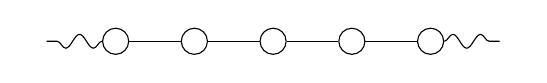
\begin{tikzpicture}[bead/.style = {draw,circle}]
\node       (0) {};
\node[bead] (1) [right of=0] {};
\node[bead] (2) [right of=1] {};
\node[bead] (3) [right of=2] {};
\node[bead] (4) [right of=3] {};
\node[bead] (5) [right of=4] {};
\node       (6) [right of=5] {};

\draw (1) -- (2);
\draw (2) -- (3);
\draw (3) -- (4);
\draw (4) -- (5);

\draw[decorate,decoration=snake] (5) -- (6);
\draw[decorate,decoration=snake] (1) -- (0);
\end{tikzpicture}\par
\end{centering}
\vspace{1em}

\noindent
Note that the beads can't slide around on the string (so the pattern ABCDE is distinct from the pattern EABCD), but you can turn any bracelet in either direction (so ABCDE is indistinguishable from EDCBA).


\section{Teamwork}

Six students are taking a taking a programming class.
There are a total of eleven programming projects, and students are required to work on these projects in groups of three.
By the end of each project, each group is unhappy, and the students never want to work in that particular group of three again (but they are willing to work with individual students they've worked with before).

Is it possible for everyone to finish the class without working in the same group twice?
If it is possible, provide a schedule; if it is impossible, give a proof.

\end{document}
